\section{Tuesday, September 12, 2023}
\subsection{Propositional Logic: Are we being limited?}
All the logic we have already discussed in class all had to revolve around propositions and their logic. However, only using propositions limits our capabilities to what we can and can't have defined at once. For example:

\begin{center}
    All men are mortal \\
    Socrates is a man \\
    $\therefore$ Socrates is a mortal.
\end{center}

The statement logic here is circumscribed by the variables we give it. "All men are mortal" is a good example here. What if we just have some man, not all? This is where \vocab{predicates} can come into play, and make our jobs easier.

\subsection{Predicates}
\textbf{\underline{Definition 5.1}}: A predicate is a sentence containing variables. To obtain a predicate, we can remove one or more nouns.

\begin{example}
    The sentence "\(x\) is greater than 3" has two parts.\\
    The first part, \(x\) is the subject. \\
    The second part, "is greater than 3" is considered the predicate.
\end{example}

With predicates, we typically assign different predicate symbols: 1. the predicate itself, and 2. the domain, or the set that the predicate variable belongs to.

\begin{example}
    Predicate: \(Q(x\)) such that \(x\) is even. \\
    Domain: \(x\) \in \mathbb{Z}
\end{example}

\subsection{Predicates with Logical Connectives}
The common logical connectives we've used (OR, AND, XOR) can be used to join predicates to make more complex predicates.

\begin{example}
    \begin{displaymath}
    T(x,y) = (A(x) \land G(x,y)) \rightarrow \neg L(y)
    \end{displaymath}
    \begin{center}
        another example being...
    \end{center}
    \begin{displaymath}
        P(x) = \neg Q(x) \lor R(x)
    \end{displaymath}
\end{example}

\subsection{Quantifiers}
So far, we've been able to figure out the truth or falsehood of statements that include variables. However, what if we expand out to see if it applies to all values in that domain, or only some? This is when we bind our variables using \vocab{quantifiers}.

\subsubsection{The Universal Quantifier}
\textbf{\underline{Definition 5.2}}: The universal quantifier "for all" $(\forall)$, says that a statement MUST be true for all values of that variable.

\begin{example}
    All humans are mortal.\\
    $\forall x$: Human(x) $\rightarrow$ Mortal(x)
\end{example}

To make the universal value explicit, we use the set notation ($\in$). Also, universal quantifiers are logically equivalent to if we put the predicate into an infinite AND connector.

\begin{example}
    $\forall x \in \mathbb{N} : P(x)$\\
    $P(0) \land P(1) \land P(2) \land $ ...
\end{example}

\subsubsection{The Existential Quantifier}
\textbf{\underline{Definition 5.3}}: The existential quantifier "there exists" $(\exists)$, says that a statement MUST be true for at LEAST one value of the variable.

\begin{example}
    There is a student is CMSC250.\\
    $\exists x \in P$: x is a student in CMSC250 where P is the set of all people. 
\end{example}

\subsection{Negations of Quantifiers}
Remember DeMorgan's laws? Well, they can also apply to quantifiers almost identically to how they applied to connectors in propositional logic. The following equivalencies hold:

\begin{center}
    $\neg \forall x: P(x) \equiv \exists x: \neg P(x)$\\
    $\neg \exists x: P(x) \equiv \forall x: \neg P(x)$
\end{center}

These are the quantifier versions of DeMorgan's laws.

\begin{example}
    \textbf{What would the negation of this be?}\\
    Every Student in your class has taken a course in Calculus.\\
    $\forall x P(x)$\\
    P(x) is the statement "x has taken a course in calculus" and $x \in $ students.
\end{example}

The negation of this statement would be "It is not the case that every student in your class has taken a course in calculus." This is also equivalent to "There is a student in your class who has not taken a course in calculus."

Do \textbf{NOT} use "none" to negate "every"!!! This is not logically equivalent, as the negation of "every" is "some".

\subsection{An Intro to Nested Quantifiers}
Quantifiers can also be nested, since predicates can take in more than one variable. Keep in mind that the order of which variable goes where DOES matter, as they may not be logically equivalent in scenarios. See the table for more.\\

\begin{center}
    \vspace{0in}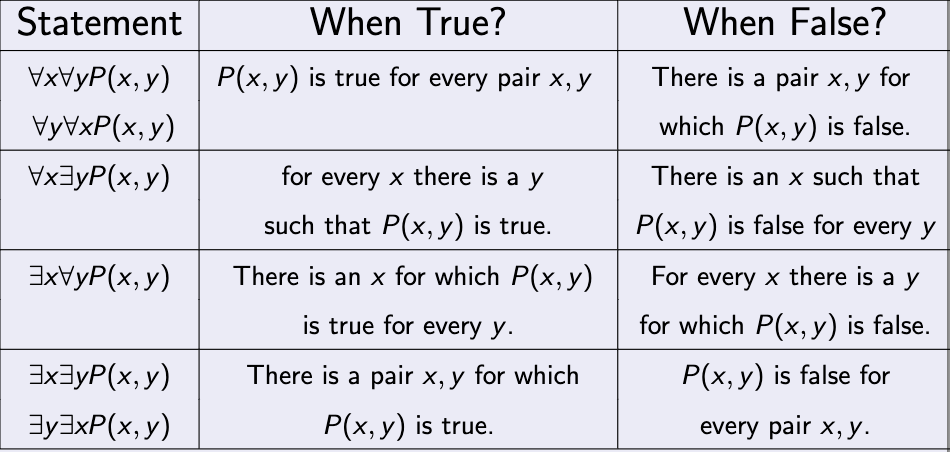
\includegraphics[scale=.7]{media/table.png} \\
\end{center}
